\documentclass[11pt, letterpaper]{article}

% Fonts and Encoding
\usepackage[utf8]{inputenc}
\usepackage[T1]{fontenc}
\usepackage{lmodern} % High-quality Latin Modern vector font

% Math and Symbols
\usepackage{amsmath, amssymb, amsthm, amsfonts, mathrsfs, mathtools}

% Layout and Geometry
\usepackage{geometry}
\geometry{letterpaper, margin=1in}
\setlength{\parindent}{0pt}
\setlength{\parskip}{0.6em}

% Formatting and Graphics
\usepackage{graphicx, xcolor, enumitem, booktabs, array, tabularx}

% TikZ for Illustrations
\usepackage{tikz}
\usetikzlibrary{arrows.meta, positioning, shapes.geometric, calc, backgrounds, matrix}

% Clickable Links and TOC
\usepackage{hyperref}
\hypersetup{
    colorlinks=true,
    linkcolor=blue,
    filecolor=magenta,      
    urlcolor=cyan,
    pdftitle={Advanced Mathematics Topic},
}

% Theorem Environments
\newtheorem{theorem}{Theorem}[section]
\newtheorem{lemma}[theorem]{Lemma}
\newtheorem{proposition}[theorem]{Proposition}
\newtheorem{corollary}[theorem]{Corollary}
\theoremstyle{definition}
\newtheorem{definition}{Definition}[section]
\newtheorem{axiom}{Axiom}[section]
\newtheorem{example}{Example}[section]
\theoremstyle{remark}
\newtheorem{remark}{Remark}[section]

% Custom Commands (Enforced standard notation)
\newcommand{\R}{\mathbb{R}}
\newcommand{\N}{\mathbb{N}}
\newcommand{\Z}{\mathbb{Z}}
\newcommand{\Q}{\mathbb{Q}}
\newcommand{\E}{\mathbb{E}}
\newcommand{\Prob}{\mathbb{P}}
\newcommand{\F}{\mathcal{F}}

\title{\textbf{Mastering Least-Squares Problems}\\ \Large A Comprehensive Guide to Orthogonality and Best Approximations}
\author{Tashfeen Omran}
\date{\today}

\begin{document}

\maketitle
\tableofcontents
\newpage

\section{Comprehensive Introduction, Context, and Prerequisites}

\subsection{Core Concepts}
In the study of linear algebra, we frequently encounter systems of linear equations of the form $A\mathbf{x} = \mathbf{b}$. When the vector $\mathbf{b}$ lies in the column space of $A$ (denoted $\text{Col } A$), the system is consistent and an exact solution exists. However, in real-world applications—such as data fitting, machine learning, and statistical modeling—systems are often overdetermined (more equations than unknowns) and inconsistent. In these cases, $\mathbf{b}$ does not lie in $\text{Col } A$, meaning no exact solution $\mathbf{x}$ exists.

The \textbf{Least-Squares Problem} asks: if we cannot find an $\mathbf{x}$ such that $A\mathbf{x} = \mathbf{b}$, can we find an $\hat{\mathbf{x}}$ that makes $A\hat{\mathbf{x}}$ as \textit{close} to $\mathbf{b}$ as possible? 

Mathematically, we seek to minimize the distance between $\mathbf{b}$ and $A\mathbf{x}$. This distance is given by the norm of the residual vector, $\|\mathbf{b} - A\mathbf{x}\|$. The term "least-squares" arises because minimizing this norm is equivalent to minimizing the sum of the squares of the components of the residual vector.

\subsection{Intuition and Derivation}
Imagine a plane representing the column space of a matrix $A$, and a vector $\mathbf{b}$ pointing out of this plane. The closest point in the plane to $\mathbf{b}$ is the orthogonal projection of $\mathbf{b}$ onto the plane, which we call $\hat{\mathbf{b}}$. 

Because $\hat{\mathbf{b}}$ is in $\text{Col } A$, there must exist some vector $\hat{\mathbf{x}}$ such that $A\hat{\mathbf{x}} = \hat{\mathbf{b}}$. Furthermore, the error vector (or residual) $\mathbf{b} - A\hat{\mathbf{x}}$ must be orthogonal to the plane $\text{Col } A$. 
By the fundamental theorem of linear algebra, a vector is orthogonal to $\text{Col } A$ if and only if it lies in the null space of $A^T$ ($\text{Nul } A^T$). Therefore:
\[ A^T (\mathbf{b} - A\hat{\mathbf{x}}) = \mathbf{0} \]
Expanding this yields the foundational equation of least-squares:
\[ A^T \mathbf{b} - A^T A \hat{\mathbf{x}} = \mathbf{0} \implies A^T A \hat{\mathbf{x}} = A^T \mathbf{b} \]
These are known as the \textbf{normal equations}.

\subsection{Historical Context and Motivation}
The method of least squares was independently developed by Carl Friedrich Gauss and Adrien-Marie Legendre in the early 19th century. The primary motivation was astronomical: predicting the orbits of celestial bodies. In 1801, the dwarf planet Ceres was discovered but soon lost behind the sun. Gauss used the least-squares method to accurately predict where Ceres would reappear, despite having only a few noisy, inconsistent observational data points. This revolutionized data analysis, proving that one could extract a highly accurate "best fit" model from overdetermined, error-prone measurements.

\subsection{Key Formulas}
\begin{itemize}
    \item \textbf{The Normal Equations:} $A^T A \hat{\mathbf{x}} = A^T \mathbf{b}$
    \item \textbf{Least-Squares Solution (if $A^T A$ is invertible):} $\hat{\mathbf{x}} = (A^T A)^{-1} A^T \mathbf{b}$
    \item \textbf{Orthogonal Projection:} $\hat{\mathbf{b}} = A\hat{\mathbf{x}}$
    \item \textbf{Least-Squares Error:} $\|\mathbf{b} - A\hat{\mathbf{x}}\|$
    \item \textbf{QR Factorization Method:} If $A = QR$, then $R\hat{\mathbf{x}} = Q^T \mathbf{b}$
\end{itemize}

\subsection{Prerequisites}
To master this topic, you must be comfortable with:
1. \textbf{Matrix Operations:} Transposition ($A^T$), matrix multiplication, and matrix inversion.
2. \textbf{Vector Spaces:} Understanding column spaces ($\text{Col } A$) and null spaces ($\text{Nul } A$).
3. \textbf{Orthogonality:} Dot products, orthogonal projections, and the Orthogonal Decomposition Theorem.
4. \textbf{QR Factorization:} Decomposing a matrix into an orthogonal matrix $Q$ and an upper triangular matrix $R$.

\newpage
\section{Detailed Homework Solutions}

\textit{Note: A strategic selection of problems has been chosen to cover every distinct problem archetype present in the chapter, ensuring comprehensive mastery without redundant repetition.}

\subsection{Problem 1: Basic Normal Equations}
\textbf{Problem Statement:} Find a least-squares solution of $A\mathbf{x} = \mathbf{b}$ by (a) constructing the normal equations for $\hat{\mathbf{x}}$ and (b) solving for $\hat{\mathbf{x}}$.
\[ A = \begin{bmatrix} 1 & 2 \\ 2 & -3 \\ -1 & 3 \end{bmatrix}, \quad \mathbf{b} = \begin{bmatrix} 4 \\ 1 \\ 2 \end{bmatrix} \]

\textbf{Solution:}
\textbf{Step 1: Compute $A^T A$.}
\[
A^T A = \begin{bmatrix} 1 & 2 & -1 \\ 2 & -3 & 3 \end{bmatrix} \begin{bmatrix} 1 & 2 \\ 2 & -3 \\ -1 & 3 \end{bmatrix}
\]
\[
A^T A = \begin{bmatrix} (1)(1) + (2)(2) + (-1)(-1) & (1)(2) + (2)(-3) + (-1)(3) \\ (2)(1) + (-3)(2) + (3)(-1) & (2)(2) + (-3)(-3) + (3)(3) \end{bmatrix}
\]
\[
A^T A = \begin{bmatrix} 1 + 4 + 1 & 2 - 6 - 3 \\ 2 - 6 - 3 & 4 + 9 + 9 \end{bmatrix} = \begin{bmatrix} 6 & -7 \\ -7 & 22 \end{bmatrix}
\]

\textbf{Step 2: Compute $A^T \mathbf{b}$.}
\[
A^T \mathbf{b} = \begin{bmatrix} 1 & 2 & -1 \\ 2 & -3 & 3 \end{bmatrix} \begin{bmatrix} 4 \\ 1 \\ 2 \end{bmatrix} = \begin{bmatrix} (1)(4) + (2)(1) + (-1)(2) \\ (2)(4) + (-3)(1) + (3)(2) \end{bmatrix} = \begin{bmatrix} 4 + 2 - 2 \\ 8 - 3 + 6 \end{bmatrix} = \begin{bmatrix} 4 \\ 11 \end{bmatrix}
\]

\textbf{Step 3: Construct the normal equations.}
\[
\begin{bmatrix} 6 & -7 \\ -7 & 22 \end{bmatrix} \begin{bmatrix} x_1 \\ x_2 \end{bmatrix} = \begin{bmatrix} 4 \\ 11 \end{bmatrix}
\]

\textbf{Step 4: Solve for $\hat{\mathbf{x}}$.}
Since $A^T A$ is a $2 \times 2$ matrix, we can use the inverse formula:
\[
(A^T A)^{-1} = \frac{1}{(6)(22) - (-7)(-7)} \begin{bmatrix} 22 & 7 \\ 7 & 6 \end{bmatrix} = \frac{1}{132 - 49} \begin{bmatrix} 22 & 7 \\ 7 & 6 \end{bmatrix} = \frac{1}{83} \begin{bmatrix} 22 & 7 \\ 7 & 6 \end{bmatrix}
\]
\[
\hat{\mathbf{x}} = \frac{1}{83} \begin{bmatrix} 22 & 7 \\ 7 & 6 \end{bmatrix} \begin{bmatrix} 4 \\ 11 \end{bmatrix} = \frac{1}{83} \begin{bmatrix} 88 + 77 \\ 28 + 66 \end{bmatrix} = \frac{1}{83} \begin{bmatrix} 165 \\ 94 \end{bmatrix} = \begin{bmatrix} 165/83 \\ 94/83 \end{bmatrix}
\]
\textbf{Final Answer:} $\hat{\mathbf{x}} = \begin{bmatrix} 165/83 \\ 94/83 \end{bmatrix}$

\vspace{1em}
\subsection{Problem 3: Normal Equations with a $4 \times 2$ Matrix}
\textbf{Problem Statement:} Find a least-squares solution of $A\mathbf{x} = \mathbf{b}$.
\[ A = \begin{bmatrix} 1 & -2 \\ -1 & 2 \\ 0 & 3 \\ 2 & 5 \end{bmatrix}, \quad \mathbf{b} = \begin{bmatrix} 3 \\ 1 \\ -4 \\ 2 \end{bmatrix} \]

\textbf{Solution:}
\textbf{Step 1: Compute $A^T A$.}
\[
A^T A = \begin{bmatrix} 1 & -1 & 0 & 2 \\ -2 & 2 & 3 & 5 \end{bmatrix} \begin{bmatrix} 1 & -2 \\ -1 & 2 \\ 0 & 3 \\ 2 & 5 \end{bmatrix} = \begin{bmatrix} 1+1+0+4 & -2-2+0+10 \\ -2-2+0+10 & 4+4+9+25 \end{bmatrix} = \begin{bmatrix} 6 & 6 \\ 6 & 42 \end{bmatrix}
\]

\textbf{Step 2: Compute $A^T \mathbf{b}$.}
\[
A^T \mathbf{b} = \begin{bmatrix} 1 & -1 & 0 & 2 \\ -2 & 2 & 3 & 5 \end{bmatrix} \begin{bmatrix} 3 \\ 1 \\ -4 \\ 2 \end{bmatrix} = \begin{bmatrix} 3 - 1 + 0 + 4 \\ -6 + 2 - 12 + 10 \end{bmatrix} = \begin{bmatrix} 6 \\ -6 \end{bmatrix}
\]

\textbf{Step 3: Solve $A^T A \hat{\mathbf{x}} = A^T \mathbf{b}$.}
\[
\begin{bmatrix} 6 & 6 \\ 6 & 42 \end{bmatrix} \begin{bmatrix} x_1 \\ x_2 \end{bmatrix} = \begin{bmatrix} 6 \\ -6 \end{bmatrix}
\]
Divide both sides by 6 to simplify:
\[
\begin{bmatrix} 1 & 1 \\ 1 & 7 \end{bmatrix} \begin{bmatrix} x_1 \\ x_2 \end{bmatrix} = \begin{bmatrix} 1 \\ -1 \end{bmatrix}
\]
Subtract Row 1 from Row 2:
\[
\begin{bmatrix} 1 & 1 \\ 0 & 6 \end{bmatrix} \begin{bmatrix} x_1 \\ x_2 \end{bmatrix} = \begin{bmatrix} 1 \\ -2 \end{bmatrix}
\]
This gives $6x_2 = -2 \implies x_2 = -1/3$.
Substitute back into Row 1: $x_1 + (-1/3) = 1 \implies x_1 = 4/3$.

\textbf{Final Answer:} $\hat{\mathbf{x}} = \begin{bmatrix} 4/3 \\ -1/3 \end{bmatrix}$

\vspace{1em}
\subsection{Problem 5: Infinite Least-Squares Solutions}
\textbf{Problem Statement:} Describe all least-squares solutions of the equation $A\mathbf{x} = \mathbf{b}$.
\[ A = \begin{bmatrix} 1 & 1 & 0 \\ 1 & 1 & 0 \\ 1 & 0 & 1 \\ 1 & 0 & 1 \end{bmatrix}, \quad \mathbf{b} = \begin{bmatrix} 1 \\ 3 \\ 8 \\ 2 \end{bmatrix} \]

\textbf{Solution:}
\textbf{Step 1: Compute $A^T A$ and $A^T \mathbf{b}$.}
\[
A^T A = \begin{bmatrix} 1 & 1 & 1 & 1 \\ 1 & 1 & 0 & 0 \\ 0 & 0 & 1 & 1 \end{bmatrix} \begin{bmatrix} 1 & 1 & 0 \\ 1 & 1 & 0 \\ 1 & 0 & 1 \\ 1 & 0 & 1 \end{bmatrix} = \begin{bmatrix} 4 & 2 & 2 \\ 2 & 2 & 0 \\ 2 & 0 & 2 \end{bmatrix}
\]
\[
A^T \mathbf{b} = \begin{bmatrix} 1 & 1 & 1 & 1 \\ 1 & 1 & 0 & 0 \\ 0 & 0 & 1 & 1 \end{bmatrix} \begin{bmatrix} 1 \\ 3 \\ 8 \\ 2 \end{bmatrix} = \begin{bmatrix} 14 \\ 4 \\ 10 \end{bmatrix}
\]

\textbf{Step 2: Set up the augmented matrix and row reduce.}
\[
\left[ \begin{array}{ccc|c} 4 & 2 & 2 & 14 \\ 2 & 2 & 0 & 4 \\ 2 & 0 & 2 & 10 \end{array} \right]
\]
Divide all rows by 2:
\[
\left[ \begin{array}{ccc|c} 2 & 1 & 1 & 7 \\ 1 & 1 & 0 & 2 \\ 1 & 0 & 1 & 5 \end{array} \right]
\]
Swap Row 1 and Row 2:
\[
\left[ \begin{array}{ccc|c} 1 & 1 & 0 & 2 \\ 2 & 1 & 1 & 7 \\ 1 & 0 & 1 & 5 \end{array} \right]
\]
$R_2 \leftarrow R_2 - 2R_1$ and $R_3 \leftarrow R_3 - R_1$:
\[
\left[ \begin{array}{ccc|c} 1 & 1 & 0 & 2 \\ 0 & -1 & 1 & 3 \\ 0 & -1 & 1 & 3 \end{array} \right]
\]
$R_3 \leftarrow R_3 - R_2$:
\[
\left[ \begin{array}{ccc|c} 1 & 1 & 0 & 2 \\ 0 & -1 & 1 & 3 \\ 0 & 0 & 0 & 0 \end{array} \right]
\]
$R_2 \leftarrow -R_2$:
\[
\left[ \begin{array}{ccc|c} 1 & 1 & 0 & 2 \\ 0 & 1 & -1 & -3 \\ 0 & 0 & 0 & 0 \end{array} \right]
\]
$R_1 \leftarrow R_1 - R_2$:
\[
\left[ \begin{array}{ccc|c} 1 & 0 & 1 & 5 \\ 0 & 1 & -1 & -3 \\ 0 & 0 & 0 & 0 \end{array} \right]
\]

\textbf{Step 3: Extract the general solution.}
The variables $x_1$ and $x_2$ are basic, while $x_3$ is free.
\[ x_1 = 5 - x_3 \]
\[ x_2 = -3 + x_3 \]
\[ x_3 \text{ is free} \]

\textbf{Final Answer:} The general least-squares solution is $\hat{\mathbf{x}} = \begin{bmatrix} 5 \\ -3 \\ 0 \end{bmatrix} + x_3 \begin{bmatrix} -1 \\ 1 \\ 1 \end{bmatrix}$.

\vspace{1em}
\subsection{Problem 9: Orthogonal Columns Shortcut}
\textbf{Problem Statement:} Find (a) the orthogonal projection of $\mathbf{b}$ onto $\text{Col } A$ and (b) a least-squares solution of $A\mathbf{x} = \mathbf{b}$.
\[ A = \begin{bmatrix} 1 & 5 \\ 3 & 1 \\ -2 & 4 \end{bmatrix}, \quad \mathbf{b} = \begin{bmatrix} 4 \\ -2 \\ -3 \end{bmatrix} \]

\textbf{Solution:}
\textbf{Step 1: Check for orthogonality.}
Let $\mathbf{a}_1 = \begin{bmatrix} 1 \\ 3 \\ -2 \end{bmatrix}$ and $\mathbf{a}_2 = \begin{bmatrix} 5 \\ 1 \\ 4 \end{bmatrix}$.
$\mathbf{a}_1 \cdot \mathbf{a}_2 = (1)(5) + (3)(1) + (-2)(4) = 5 + 3 - 8 = 0$.
Since the columns are orthogonal, $A^T A$ will be a diagonal matrix, simplifying calculations immensely.

\textbf{Step 2: Compute $A^T A$ and $A^T \mathbf{b}$.}
\[
A^T A = \begin{bmatrix} \mathbf{a}_1 \cdot \mathbf{a}_1 & 0 \\ 0 & \mathbf{a}_2 \cdot \mathbf{a}_2 \end{bmatrix} = \begin{bmatrix} 1^2 + 3^2 + (-2)^2 & 0 \\ 0 & 5^2 + 1^2 + 4^2 \end{bmatrix} = \begin{bmatrix} 14 & 0 \\ 0 & 42 \end{bmatrix}
\]
\[
A^T \mathbf{b} = \begin{bmatrix} \mathbf{a}_1 \cdot \mathbf{b} \\ \mathbf{a}_2 \cdot \mathbf{b} \end{bmatrix} = \begin{bmatrix} (1)(4) + (3)(-2) + (-2)(-3) \\ (5)(4) + (1)(-2) + (4)(-3) \end{bmatrix} = \begin{bmatrix} 4 - 6 + 6 \\ 20 - 2 - 12 \end{bmatrix} = \begin{bmatrix} 4 \\ 6 \end{bmatrix}
\]

\textbf{Step 3: Solve for $\hat{\mathbf{x}}$.}
\[
\begin{bmatrix} 14 & 0 \\ 0 & 42 \end{bmatrix} \begin{bmatrix} x_1 \\ x_2 \end{bmatrix} = \begin{bmatrix} 4 \\ 6 \end{bmatrix} \implies x_1 = \frac{4}{14} = \frac{2}{7}, \quad x_2 = \frac{6}{42} = \frac{1}{7}
\]
So, $\hat{\mathbf{x}} = \begin{bmatrix} 2/7 \\ 1/7 \end{bmatrix}$.

\textbf{Step 4: Compute the orthogonal projection $\hat{\mathbf{b}}$.}
\[
\hat{\mathbf{b}} = A\hat{\mathbf{x}} = \frac{2}{7} \begin{bmatrix} 1 \\ 3 \\ -2 \end{bmatrix} + \frac{1}{7} \begin{bmatrix} 5 \\ 1 \\ 4 \end{bmatrix} = \begin{bmatrix} 2/7 + 5/7 \\ 6/7 + 1/7 \\ -4/7 + 4/7 \end{bmatrix} = \begin{bmatrix} 1 \\ 1 \\ 0 \end{bmatrix}
\]

\textbf{Final Answer:} (a) $\hat{\mathbf{b}} = \begin{bmatrix} 1 \\ 1 \\ 0 \end{bmatrix}$, (b) $\hat{\mathbf{x}} = \begin{bmatrix} 2/7 \\ 1/7 \end{bmatrix}$.

\vspace{1em}
\subsection{Problem 15: Using QR Factorization}
\textbf{Problem Statement:} Use the factorization $A = QR$ to find the least-squares solution of $A\mathbf{x} = \mathbf{b}$.
\[ A = \begin{bmatrix} 2 & 3 \\ 2 & 4 \\ 1 & 1 \end{bmatrix} = \begin{bmatrix} 2/3 & -1/3 \\ 2/3 & 2/3 \\ 1/3 & -2/3 \end{bmatrix} \begin{bmatrix} 3 & 5 \\ 0 & 1 \end{bmatrix}, \quad \mathbf{b} = \begin{bmatrix} 7 \\ 3 \\ 1 \end{bmatrix} \]

\textbf{Solution:}
By Theorem 15, the least-squares solution satisfies $R\hat{\mathbf{x}} = Q^T \mathbf{b}$.

\textbf{Step 1: Compute $Q^T \mathbf{b}$.}
\[
Q^T \mathbf{b} = \begin{bmatrix} 2/3 & 2/3 & 1/3 \\ -1/3 & 2/3 & -2/3 \end{bmatrix} \begin{bmatrix} 7 \\ 3 \\ 1 \end{bmatrix} = \begin{bmatrix} \frac{14}{3} + \frac{6}{3} + \frac{1}{3} \\[4pt] -\frac{7}{3} + \frac{6}{3} - \frac{2}{3} \end{bmatrix} = \begin{bmatrix} 21/3 \\ -3/3 \end{bmatrix} = \begin{bmatrix} 7 \\ -1 \end{bmatrix}
\]

\textbf{Step 2: Solve $R\hat{\mathbf{x}} = Q^T \mathbf{b}$.}
\[
\begin{bmatrix} 3 & 5 \\ 0 & 1 \end{bmatrix} \begin{bmatrix} x_1 \\ x_2 \end{bmatrix} = \begin{bmatrix} 7 \\ -1 \end{bmatrix}
\]
Using back-substitution:
From the second row: $x_2 = -1$.
From the first row: $3x_1 + 5(-1) = 7 \implies 3x_1 = 12 \implies x_1 = 4$.

\textbf{Final Answer:} $\hat{\mathbf{x}} = \begin{bmatrix} 4 \\ -1 \end{bmatrix}$.

\vspace{1em}
\subsection{Problem 27: Theoretical Proof on Null Spaces}
\textbf{Problem Statement:} Let $A$ be an $m \times n$ matrix. Show that a vector $\mathbf{x}$ in $\R^n$ satisfies $A\mathbf{x} = \mathbf{0}$ if and only if $A^T A \mathbf{x} = \mathbf{0}$. This shows that $\text{Nul } A = \text{Nul } A^T A$.

\textbf{Solution:}
\textbf{Part (a): Show that if $A\mathbf{x} = \mathbf{0}$, then $A^T A \mathbf{x} = \mathbf{0}$.}
Assume $\mathbf{x} \in \text{Nul } A$. Then $A\mathbf{x} = \mathbf{0}$.
Multiply both sides on the left by $A^T$:
\[ A^T (A\mathbf{x}) = A^T (\mathbf{0}) \implies A^T A \mathbf{x} = \mathbf{0} \]
Thus, $\mathbf{x} \in \text{Nul } A^T A$.

\textbf{Part (b): Show that if $A^T A \mathbf{x} = \mathbf{0}$, then $A\mathbf{x} = \mathbf{0}$.}
Assume $\mathbf{x} \in \text{Nul } A^T A$. Then $A^T A \mathbf{x} = \mathbf{0}$.
Multiply both sides on the left by $\mathbf{x}^T$:
\[ \mathbf{x}^T (A^T A \mathbf{x}) = \mathbf{x}^T \mathbf{0} \implies (\mathbf{x}^T A^T) (A\mathbf{x}) = 0 \]
By the properties of transposes, $\mathbf{x}^T A^T = (A\mathbf{x})^T$. Therefore:
\[ (A\mathbf{x})^T (A\mathbf{x}) = 0 \]
The expression $(A\mathbf{x})^T (A\mathbf{x})$ is exactly the dot product of $A\mathbf{x}$ with itself, which is $\|A\mathbf{x}\|^2$.
\[ \|A\mathbf{x}\|^2 = 0 \]
By the positive definite property of vector norms, the norm of a vector is zero if and only if the vector itself is the zero vector.
\[ A\mathbf{x} = \mathbf{0} \]
Thus, $\mathbf{x} \in \text{Nul } A$. Since both directions hold, $\text{Nul } A = \text{Nul } A^T A$.

\newpage
\section{In-Depth Analysis of Problems and Techniques}

\subsection{Problem Types and General Approach}
\renewcommand{\arraystretch}{1.5}
\begin{tabularx}{\textwidth}{>{\raggedright\arraybackslash}p{4cm} X}
\toprule
\textbf{Problem Archetype} & \textbf{General Strategy} \\
\midrule
\textbf{Basic Normal Equations} \newline (e.g., Problems 1, 3) & Compute $A^T A$ and $A^T \mathbf{b}$. Set up the system $A^T A \hat{\mathbf{x}} = A^T \mathbf{b}$. If $A^T A$ is $2 \times 2$, use the determinant-based inverse formula. Otherwise, use Gaussian elimination. \\
\addlinespace[4pt]
\textbf{Infinite Solutions} \newline (e.g., Problem 5) & Occurs when the columns of $A$ are linearly dependent, making $A^T A$ non-invertible. Set up the augmented matrix $[A^T A \mid A^T \mathbf{b}]$, row reduce to RREF, and express the solution parametrically with free variables. \\
\addlinespace[4pt]
\textbf{Orthogonal Columns} \newline (e.g., Problem 9) & If the columns of $A$ are orthogonal, $A^T A$ is a diagonal matrix. The system decouples, and you can solve for each component of $\hat{\mathbf{x}}$ independently using $\hat{x}_i = \frac{\mathbf{a}_i \cdot \mathbf{b}}{\mathbf{a}_i \cdot \mathbf{a}_i}$. \\
\addlinespace[4pt]
\textbf{QR Factorization} \newline (e.g., Problem 15) & Avoid computing $A^T A$ entirely. Instead, compute $Q^T \mathbf{b}$. Then, solve the upper triangular system $R\hat{\mathbf{x}} = Q^T \mathbf{b}$ using simple back-substitution. This is numerically more stable. \\
\bottomrule
\end{tabularx}

\subsection{Key Algebraic and Calculus Manipulations}
\begin{itemize}
    \item \textbf{The Transpose Distribution Trick:} In theoretical proofs (like Problem 27), recognizing that $\mathbf{x}^T A^T A \mathbf{x}$ can be rewritten as $(A\mathbf{x})^T (A\mathbf{x})$ is a critical algebraic manipulation. It transforms a matrix multiplication problem into a vector norm problem ($\|A\mathbf{x}\|^2$), allowing us to conclude that $A\mathbf{x} = \mathbf{0}$.
    \item \textbf{Back-Substitution with $R$:} In QR factorization problems, the matrix $R$ is always upper triangular. The manipulation trick here is to \textit{never} find $R^{-1}$. Instead, write out the system of equations starting from the bottom row (which will only have one variable) and substitute upwards.
    \item \textbf{Decoupling via Orthogonality:} When columns are orthogonal, the off-diagonal elements of $A^T A$ become zero. This algebraic simplification reduces an $n \times n$ system of equations into $n$ independent scalar equations, drastically reducing computational complexity.
\end{itemize}

\newpage
\section{"Cheatsheet" and Tips for Success}

\subsection{Core Formulas}
\renewcommand{\arraystretch}{1.5}
\begin{tabularx}{\textwidth}{>{\raggedright\arraybackslash}p{5cm} >{$\displaystyle}X<{$}}
\toprule
\textbf{Concept} & \textbf{Formula} \\
\midrule
Normal Equations & A^T A \hat{\mathbf{x}} = A^T \mathbf{b} \\
Least-Squares Solution & \hat{\mathbf{x}} = (A^T A)^{-1} A^T \mathbf{b} \quad \text{(if columns of } A \text{ are independent)} \\
Orthogonal Projection & \hat{\mathbf{b}} = A\hat{\mathbf{x}} \\
Least-Squares Error & \|\mathbf{b} - A\hat{\mathbf{x}}\| = \sqrt{(\mathbf{b} - \hat{\mathbf{b}})^T (\mathbf{b} - \hat{\mathbf{b}})} \\
QR Method & R\hat{\mathbf{x}} = Q^T \mathbf{b} \\
\bottomrule
\end{tabularx}

\subsection{Visualizing the Least-Squares Projection}
The following diagram illustrates the geometric intuition behind the least-squares problem. We project $\mathbf{b}$ orthogonally onto the column space of $A$.

\begin{center}
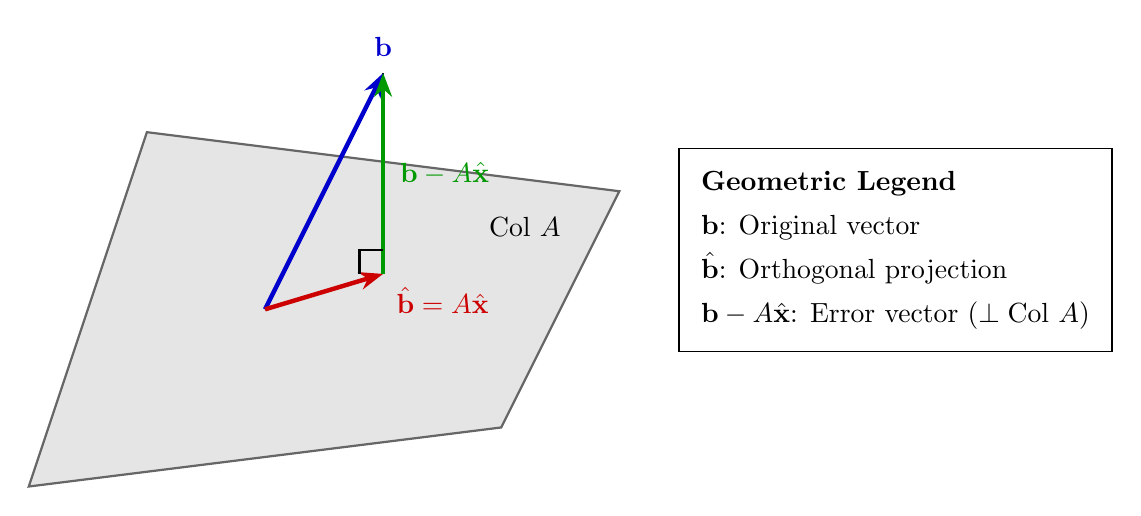
\begin{tikzpicture}[scale=1.5]
    % Draw the plane representing Col A
    \fill[gray!20] (-1,-1) -- (3,-0.5) -- (4,1.5) -- (0,2) -- cycle;
    \draw[thick, gray!80!black] (-1,-1) -- (3,-0.5) -- (4,1.5) -- (0,2) -- cycle;
    
    % Draw vectors
    \coordinate (O) at (1, 0.5);
    \coordinate (b) at (2, 2.5);
    \coordinate (bhat) at (2, 0.8);
    
    % Draw projection line
    \draw[dashed, thick] (b) -- (bhat);
    
    % Draw vectors from origin
    \draw[ultra thick, -{Stealth[length=3mm]}, blue!80!black] (O) -- (b) node[above=2pt] {$\mathbf{b}$};
    \draw[ultra thick, -{Stealth[length=3mm]}, red!80!black] (O) -- (bhat) node[below right=1pt] {$\hat{\mathbf{b}} = A\hat{\mathbf{x}}$};
    
    % Draw error vector
    \draw[ultra thick, -{Stealth[length=3mm]}, green!60!black] (bhat) -- (b) node[midway, right=2pt] {$\mathbf{b} - A\hat{\mathbf{x}}$};
    
    % Right angle square
    \draw[thick] (2, 1.0) -- (1.8, 1.0) -- (1.8, 0.8);
    
    % Labels
    \node[black] at (3.2, 1.2) {$\text{Col } A$};
    
    % Legend using single-node multiline rule
    \node[align=left, anchor=west, draw, inner sep=8pt, fill=white] at (4.5, 1) {
        \textbf{Geometric Legend}\\[4pt]
        $\mathbf{b}$: Original vector\\[4pt]
        $\hat{\mathbf{b}}$: Orthogonal projection\\[4pt]
        $\mathbf{b} - A\hat{\mathbf{x}}$: Error vector ($\perp \text{Col } A$)
    };
\end{tikzpicture}
\end{center}

\subsection{Tips and Common Pitfalls}
\begin{itemize}
    \item \textbf{Cheat:} If a problem asks for the least-squares error, you \textit{must} compute $\hat{\mathbf{b}} = A\hat{\mathbf{x}}$ first. The error is the magnitude of the difference between the original $\mathbf{b}$ and the projected $\hat{\mathbf{b}}$.
    \item \textbf{Pitfall 1:} Confusing $\hat{\mathbf{x}}$ with $\hat{\mathbf{b}}$. $\hat{\mathbf{x}}$ is the vector of weights (in $\R^n$) that multiplies the columns of $A$. $\hat{\mathbf{b}}$ is the actual projected vector (in $\R^m$).
    \item \textbf{Pitfall 2:} Assuming $A^T A$ is always invertible. It is only invertible if the columns of $A$ are linearly independent. If they are dependent, you must use row reduction on the augmented matrix $[A^T A \mid A^T \mathbf{b}]$ to find the general solution.
    \item \textbf{Pitfall 3:} Forgetting to transpose $A$ when setting up the normal equations. Always double-check that you are computing $A^T A$, not $A A^T$.
\end{itemize}

\newpage
\section{Conceptual Synthesis and The "Big Picture"}

\subsection{Thematic Connections}
The core theme of the least-squares problem is \textbf{optimization via orthogonal projection}. This theme appears repeatedly across mathematics:
*   \textbf{Calculus:} Finding the minimum of a function by setting its derivative to zero is analogous to finding the minimum distance by ensuring the error vector is orthogonal (derivative of the squared error with respect to $\mathbf{x}$ is zero).
*   \textbf{Fourier Series:} Approximating a continuous function with a finite sum of sines and cosines is exactly an infinite-dimensional least-squares problem, where we project a function onto an orthogonal basis of trigonometric functions.

\subsection{Forward and Backward Links}
*   \textbf{Backward Link:} This topic is the logical culmination of earlier linear algebra concepts. It unifies matrix multiplication, transposes, null spaces, column spaces, and orthogonality into a single, powerful applied framework.
*   \textbf{Forward Link:} Least-squares is the absolute bedrock of \textbf{Statistical Regression} and \textbf{Machine Learning}. Every time a data scientist fits a linear regression model to data, they are solving $A^T A \hat{\mathbf{x}} = A^T \mathbf{b}$ under the hood. Furthermore, understanding how $A^T A$ behaves is crucial for advanced topics like Principal Component Analysis (PCA) and Singular Value Decomposition (SVD).

\section{Abstract Real-World Modeling (AI, ML, \& Quant Finance)}

\subsection{Concrete Scenarios}
1. \textbf{Quantitative Finance (Factor Modeling):} In Arbitrage Pricing Theory (APT), quants model the expected return of an asset as a linear combination of various macroeconomic factors (e.g., GDP growth, inflation, market risk premium). Because market data is noisy, the system is overdetermined, and least-squares is used to estimate the asset's sensitivity (Beta) to each factor.
2. \textbf{Machine Learning (Linear Regression):} In supervised learning, an AI is trained to predict a continuous target variable (like housing prices) based on input features (square footage, number of bedrooms). The training process involves finding the optimal weights that minimize the Mean Squared Error (MSE) over the training dataset—a direct application of the normal equations.

\subsection{Model Problem Setup: Multi-Factor Asset Pricing}
Let us formulate a rigorous mathematical model for estimating factor betas in Quantitative Finance.

\textbf{State Space and Variables:}
Let $N$ be the number of historical trading days observed.
Let $\mathbf{r} \in \R^N$ be the vector of excess returns for a specific stock (e.g., Apple) over the risk-free rate.
Let $K$ be the number of risk factors. We define a design matrix $F \in \R^{N \times K}$, where each column represents the historical returns of a specific factor portfolio (e.g., Market, Size, Value).
Let $\boldsymbol{\beta} \in \R^K$ be the unknown vector of factor loadings (sensitivities) we wish to estimate.
Let $\boldsymbol{\epsilon} \in \R^N$ be the stochastic noise vector, assumed to be independent and identically distributed (i.i.d.) with $\E[\boldsymbol{\epsilon}] = \mathbf{0}$ and $\text{Var}(\boldsymbol{\epsilon}) = \sigma^2 I$.

\textbf{The Stochastic Model:}
The return generating process is modeled as:
\[ \mathbf{r} = F\boldsymbol{\beta} + \boldsymbol{\epsilon} \]

\textbf{Optimization Problem:}
To find the optimal factor loadings $\hat{\boldsymbol{\beta}}$, we define a Loss Function $\mathcal{L}(\boldsymbol{\beta})$ based on the $L_2$ norm of the residuals:
\[ \mathcal{L}(\boldsymbol{\beta}) = \|\mathbf{r} - F\boldsymbol{\beta}\|^2 = (\mathbf{r} - F\boldsymbol{\beta})^T (\mathbf{r} - F\boldsymbol{\beta}) \]
To minimize this loss function, we take the gradient with respect to $\boldsymbol{\beta}$ and set it to the zero vector:
\[ \nabla_{\boldsymbol{\beta}} \mathcal{L} = -2F^T \mathbf{r} + 2F^T F \boldsymbol{\beta} = \mathbf{0} \]
This rigorously derives the normal equations in a financial context:
\[ F^T F \hat{\boldsymbol{\beta}} = F^T \mathbf{r} \]
Assuming the factor portfolios are linearly independent (no perfect multicollinearity), $F^T F$ is positive definite and invertible, yielding the Ordinary Least Squares (OLS) estimator:
\[ \hat{\boldsymbol{\beta}} = (F^T F)^{-1} F^T \mathbf{r} \]

\newpage
\section{Common Variations and Untested Concepts}

While the provided homework covers standard least-squares, a critical variation used in modern applications is \textbf{Tikhonov Regularization (Ridge Regression)}. 

\subsection{Concept: Ridge Regression}
When the columns of $A$ are nearly linearly dependent (multicollinearity), the matrix $A^T A$ becomes ill-conditioned. Its determinant is close to zero, making the inverse $(A^T A)^{-1}$ highly sensitive to small changes in data, leading to massive, unstable weights in $\hat{\mathbf{x}}$.
To fix this, we add a small "penalty" term $\lambda > 0$ to the diagonal of $A^T A$. The modified normal equations become:
\[ (A^T A + \lambda I) \hat{\mathbf{x}}_{\text{ridge}} = A^T \mathbf{b} \]
This guarantees the matrix is invertible and shrinks the coefficients, preventing overfitting in machine learning models.

\subsection{Worked Example}
Let $A = \begin{bmatrix} 1 & 1 \\ 1 & 1.01 \\ 1 & 1 \end{bmatrix}$ and $\mathbf{b} = \begin{bmatrix} 2 \\ 3 \\ 2 \end{bmatrix}$. Notice the columns of $A$ are almost identical.
\[ A^T A = \begin{bmatrix} 3 & 3.01 \\ 3.01 & 3.0201 \end{bmatrix} \]
The determinant is $(3)(3.0201) - (3.01)^2 = 9.0603 - 9.0601 = 0.0002$. This is dangerously close to zero.
If we apply Ridge Regression with $\lambda = 0.1$:
\[ A^T A + \lambda I = \begin{bmatrix} 3 & 3.01 \\ 3.01 & 3.0201 \end{bmatrix} + \begin{bmatrix} 0.1 & 0 \\ 0 & 0.1 \end{bmatrix} = \begin{bmatrix} 3.1 & 3.01 \\ 3.01 & 3.1201 \end{bmatrix} \]
The new determinant is $(3.1)(3.1201) - (3.01)^2 = 9.67231 - 9.0601 = 0.61221$. The matrix is now well-conditioned and easily invertible, yielding a stable, robust solution.

\newpage
\section{Advanced Diagnostic Testing: "Find the Flaw"}

Below are five problems with step-by-step solutions that contain a single, critical flaw. Your task as a student is to identify the error, explain why it is wrong, and provide the correct solution.

\subsection{Problem 1: The Normal Equation Setup}
\textbf{Question:} Find the least-squares solution for $A = \begin{bmatrix} 1 & 1 \\ 1 & -1 \\ 1 & 1 \end{bmatrix}$ and $\mathbf{b} = \begin{bmatrix} 2 \\ 0 \\ 2 \end{bmatrix}$.

\textbf{Flawed Solution:}
To find the least-squares solution, we use the normal equations. First, compute $A A^T$:
\[ A A^T = \begin{bmatrix} 1 & 1 \\ 1 & -1 \\ 1 & 1 \end{bmatrix} \begin{bmatrix} 1 & 1 & 1 \\ 1 & -1 & 1 \end{bmatrix} = \begin{bmatrix} 2 & 0 & 2 \\ 0 & 2 & 0 \\ 2 & 0 & 2 \end{bmatrix} \]
Next, we solve $A A^T \hat{\mathbf{x}} = A \mathbf{b}$.
\textbf{Flaw to find:} Look closely at the matrix multiplication order in the normal equations.

\subsection{Problem 2: Calculating the Error}
\textbf{Question:} Find the least-squares error for $A = \begin{bmatrix} 1 \\ 2 \end{bmatrix}$ and $\mathbf{b} = \begin{bmatrix} 3 \\ 1 \end{bmatrix}$.

\textbf{Flawed Solution:}
$A^T A = [1^2 + 2^2] = [5]$.
$A^T \mathbf{b} = (1)(3) + (2)(1) = 5$.
Solving $5\hat{x} = 5 \implies \hat{x} = 1$.
The least-squares error is the distance between $\mathbf{b}$ and $\hat{x}$:
\[ \text{Error} = \|\mathbf{b} - \hat{x}\| = \left\| \begin{bmatrix} 3 \\ 1 \end{bmatrix} - 1 \right\| = \left\| \begin{bmatrix} 2 \\ 0 \end{bmatrix} \right\| = 2 \]
\textbf{Flaw to find:} What space does $\hat{x}$ live in compared to $\mathbf{b}$? Can you subtract a scalar from a vector?

\subsection{Problem 3: QR Factorization Mix-up}
\textbf{Question:} A matrix $A$ has a QR factorization where $R = \begin{bmatrix} 2 & 1 \\ 0 & 3 \end{bmatrix}$. For a vector $\mathbf{b}$, we are given $Q^T \mathbf{b} = \begin{bmatrix} 4 \\ 6 \end{bmatrix}$. Find the least-squares solution.

\textbf{Flawed Solution:}
By Theorem 15, the least-squares solution is found by solving $R^T \hat{\mathbf{x}} = Q^T \mathbf{b}$.
\[ \begin{bmatrix} 2 & 0 \\ 1 & 3 \end{bmatrix} \begin{bmatrix} x_1 \\ x_2 \end{bmatrix} = \begin{bmatrix} 4 \\ 6 \end{bmatrix} \]
From row 1: $2x_1 = 4 \implies x_1 = 2$.
From row 2: $1(2) + 3x_2 = 6 \implies 3x_2 = 4 \implies x_2 = 4/3$.
\textbf{Flaw to find:} Check the exact formula for solving least-squares using QR factorization.

\subsection{Problem 4: The Orthogonal Shortcut Trap}
\textbf{Question:} Find the orthogonal projection of $\mathbf{b} = \begin{bmatrix} 1 \\ 1 \\ 1 \end{bmatrix}$ onto the column space of $A = \begin{bmatrix} 1 & 1 \\ 1 & 2 \\ 1 & 3 \end{bmatrix}$.

\textbf{Flawed Solution:}
Let $\mathbf{a}_1 = \begin{bmatrix} 1 \\ 1 \\ 1 \end{bmatrix}$ and $\mathbf{a}_2 = \begin{bmatrix} 1 \\ 2 \\ 3 \end{bmatrix}$.
We can project $\mathbf{b}$ directly onto the columns:
\[ \hat{\mathbf{b}} = \frac{\mathbf{b} \cdot \mathbf{a}_1}{\mathbf{a}_1 \cdot \mathbf{a}_1} \mathbf{a}_1 + \frac{\mathbf{b} \cdot \mathbf{a}_2}{\mathbf{a}_2 \cdot \mathbf{a}_2} \mathbf{a}_2 \]
$\mathbf{b} \cdot \mathbf{a}_1 = 3$, $\mathbf{a}_1 \cdot \mathbf{a}_1 = 3$.
$\mathbf{b} \cdot \mathbf{a}_2 = 6$, $\mathbf{a}_2 \cdot \mathbf{a}_2 = 14$.
\[ \hat{\mathbf{b}} = \frac{3}{3} \begin{bmatrix} 1 \\ 1 \\ 1 \end{bmatrix} + \frac{6}{14} \begin{bmatrix} 1 \\ 2 \\ 3 \end{bmatrix} = \begin{bmatrix} 10/7 \\ 13/7 \\ 16/7 \end{bmatrix} \]
\textbf{Flaw to find:} When is this specific projection formula valid? Check the relationship between $\mathbf{a}_1$ and $\mathbf{a}_2$.

\subsection{Problem 5: The Invertibility Assumption}
\textbf{Question:} Find the least-squares solution for $A = \begin{bmatrix} 1 & 2 \\ 2 & 4 \\ 3 & 6 \end{bmatrix}$ and $\mathbf{b} = \begin{bmatrix} 1 \\ 1 \\ 1 \end{bmatrix}$.

\textbf{Flawed Solution:}
$A^T A = \begin{bmatrix} 1 & 2 & 3 \\ 2 & 4 & 6 \end{bmatrix} \begin{bmatrix} 1 & 2 \\ 2 & 4 \\ 3 & 6 \end{bmatrix} = \begin{bmatrix} 14 & 28 \\ 28 & 56 \end{bmatrix}$.
$A^T \mathbf{b} = \begin{bmatrix} 1 & 2 & 3 \\ 2 & 4 & 6 \end{bmatrix} \begin{bmatrix} 1 \\ 1 \\ 1 \end{bmatrix} = \begin{bmatrix} 6 \\ 12 \end{bmatrix}$.
The solution is $\hat{\mathbf{x}} = (A^T A)^{-1} A^T \mathbf{b}$.
\[ (A^T A)^{-1} = \frac{1}{(14)(56) - (28)(28)} \begin{bmatrix} 56 & -28 \\ -28 & 14 \end{bmatrix} = \frac{1}{784 - 784} \begin{bmatrix} 56 & -28 \\ -28 & 14 \end{bmatrix} \]
Since the determinant is 0, the least-squares solution does not exist.
\textbf{Flaw to find:} Does a determinant of 0 mean the least-squares solution doesn't exist, or does it mean something else about the nature of the solutions?

\end{document}